\documentclass[a4paper]{article}
\usepackage{student}

% Metadata
\date{\today}
\setmodule{CS110: Computer Architecture}
\setterm{Spring, 2024}

%-------------------------------%
% Other details
% TODO: Fill these
%-------------------------------%
\title{Assignment 4: Digital circuit}
\setmembername{}  % Fill student name
\setmemberuid{}  % Fill  student id

%-------------------------------%
% Add / Delete commands and packages
% TODO: Add / Delete here as you need
%-------------------------------%
\usepackage{amsmath,amssymb,bm}
\usepackage{hyperref}

\newcommand{\KL}{\mathrm{KL}}
\newcommand{\R}{\mathbb{R}}
\newcommand{\E}{\mathbb{E}}
\newcommand{\T}{\top}

\newcommand{\expdist}[2]{%
        \normalfont{\textsc{Exp}}(#1, #2)%
    }
\newcommand{\expparam}{\bm \lambda}
\newcommand{\Expparam}{\bm \Lambda}
\newcommand{\natparam}{\bm \eta}
\newcommand{\Natparam}{\bm H}
\newcommand{\sufstat}{\bm u}

% Main document
\begin{document}
    % Add header
    \header{}
\textcolor{red}{\textbf{Attention: }}
\textbf{Recommend using \LaTeX to complete your work. You can use any tool, such as Logisim, Visio, Draw.io, PowerPoint, etc., to create diagrams. However, handwritten or hand-drawn content is not acceptable.}

\section{Combinational logic}
Analyze the circuit shown in Fig.~\ref{fig:circuit} and answer the following questions:
\begin{figure}[htbp]
    \centering
    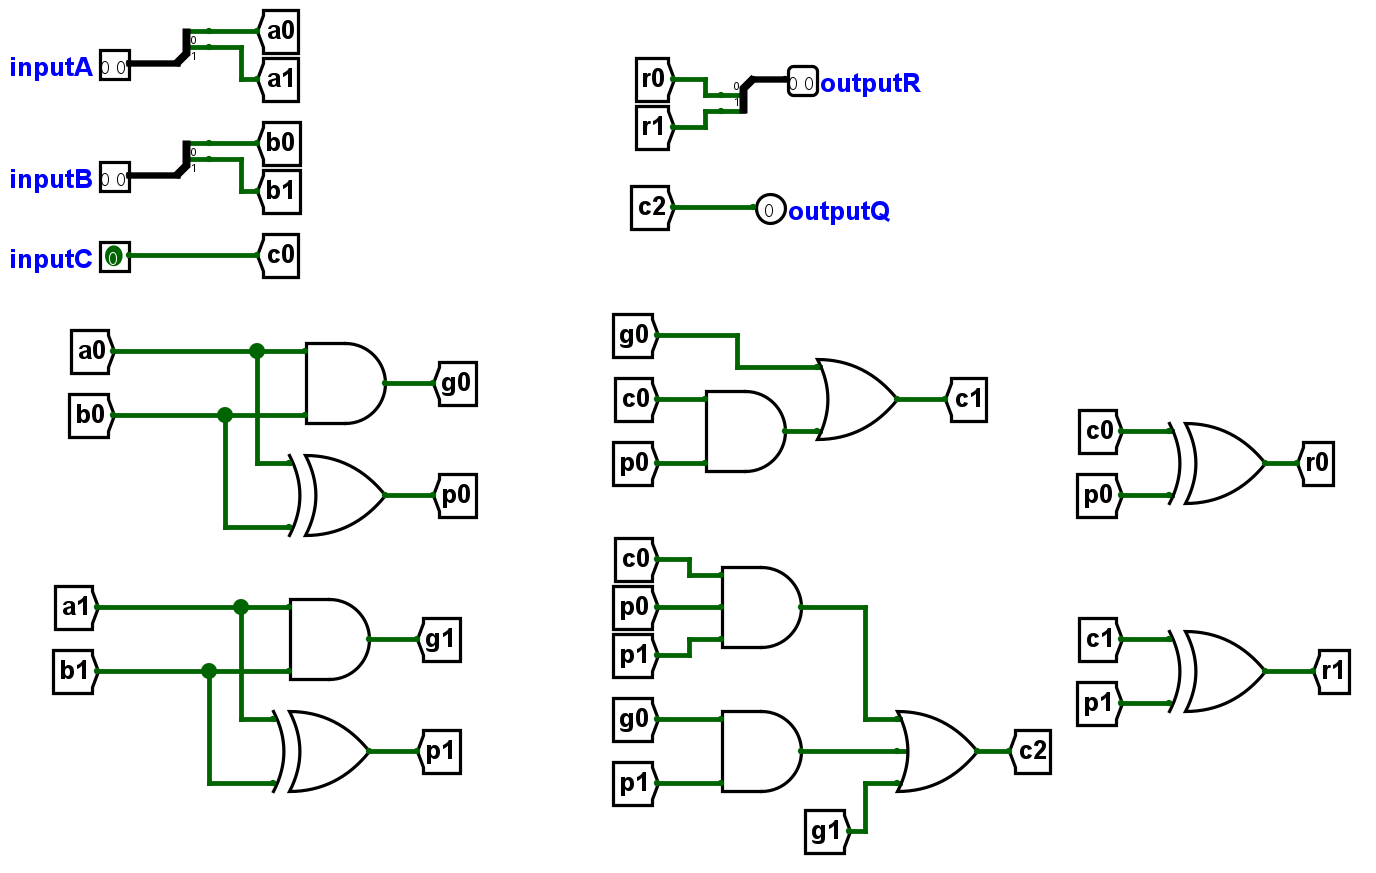
\includegraphics[width=0.8\textwidth]{circuit.png}
    \caption{A 2-bit arithmetic circuit}
    \label{fig:circuit}
\end{figure}

(a) Draw the truth table of this circuit.\textbf{[10 pt]}

(b) Which kind of arithmetic operation (addition, subtraction, multiplication, division, shift, or comparison) is performed by this circuit? What are the advantages and disadvantages of the circuit in Fig.~\ref{fig:circuit} compared to the corresponding arithmetic circuit mentioned in \href{https://toast-lab.sist.shanghaitech.edu.cn/courses/CS110@ShanghaiTech/Spring-2024/lecture_notes/L09.\%20Digital\%20circuits\%20and\%20systems\%201.pdf}{Digital circuits I}?\textbf{[10 pt]}

(b) Assume that all 2-input logic gates have 1 ns delay, all 3-input logic gates have 2 ns delay, and other delays are not considered. Calculate the max delay of this circuit.\textbf{[10 pt]}

\begin{answer}[Question 1]
        Your answer here.
\end{answer}

\newpage
\section{SDS}
Draw a counter that counts from 0 to 5 using three D flip-flops (each flip-flops represents one output bit) and some 2-input logic gates (AND, OR, NOT). Please use the method taught in class to build a Moore FSM that implements the circular counter. Complete the state transition logic and output logic. \textbf{[35 pt]}
\begin{figure}[hp]
    \centering
    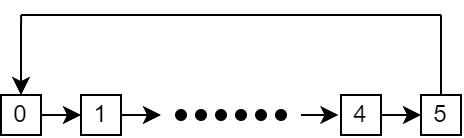
\includegraphics[height=2cm]{q2.png}
    \caption{The counter cycles through the process of counting from 0 to 5.}
    \label{fig:q2}
\end{figure}
\begin{answer}[Question 2]
        Your answer here.
\end{answer}

\newpage
\section{Finite state machine}

The function of a vending machine which sells bottles of soda is described below:

\begin{itemize}
\item[$\bullet$] Each bottle costs \$1.50. 
\item[$\bullet$] The machine only accepts \$0.50 and \$1 coins. If a customer inserts enough coins, the machine will dispense a bottle of soda (FSM will output ``1", otherwise ``0'') and returns change if needed , e.g., the output of DISPENSE states may be ``1 \$0.5", other states' output may be ``0 \$0''.
\item[$\bullet$] The process happens one coin at a time, and there is no simultaneous insertion of multiple coins or shipping of multiple bottles. After each transaction, the vending machine enters the IDLE state.
\item[$\bullet$] We don’t need to account for a scenario where a customer inserts coins but decides not to make a purchase.
\end{itemize}


(a) Draw the FSM (Moore machine) for this vending machine.\textbf{[15 pt]}

(b) Draw the FSM (Mealy machine) for this vending machine.\textbf{[10 pt]}

(c) Could Moore machines and Mealy machines be converted into each other to implement the same function? Compare their difference.\textbf{[10 pt]}
\begin{answer}[Question 3]
        Your answer here.
\end{answer}

\end{document}
